\documentclass[border=3mm,preview]{standalone}
\usepackage[]{graphicx}\usepackage[]{color}

\usepackage{alltt}\usepackage[]{graphicx}\usepackage[]{color}
\usepackage[utf8]{inputenc}
\usepackage[spanish]{babel}
\usepackage{fancyhdr}
\usepackage{lastpage}
\usepackage{lscape} %Para seleccionar páginas horizontales 
\usepackage[cc]{titlepic} 
\usepackage[hidelinks]{hyperref}  %Para links ocultos
\usepackage{url} %Para direcciones web
\usepackage[makeroom]{cancel}
\pagestyle{fancy}
\usepackage{multicol} % muchas columnas
\usepackage{booktabs} % midrule, bottomrule
\usepackage{titlesec} % cambiar secuencias de TOC 
\usepackage{siunitx}
\usepackage{varwidth} % PAra los documentos standalone y el ajuste preciso
\usepackage{subcaption} % Para usar subcaptions en las matrices de imágenes 
\sisetup{binary-units = true,table-format=7.0}
\let\bold\boldsymbol
\let\bf\mathbf


\fancyhf{}
 \setcounter{page}{1}
%\rfoot{Página \thepage \hspace{1pt} de \pageref{LastPage}}
\setcounter{section}{0}

\usepackage{blindtext}  %Texo sin sentido
\usepackage{amsmath} \newenvironment{smatrix}{\left(\begin{smallmatrix}}{\end{smallmatrix}\right)} %SMALL
\usepackage{amsthm}
\usepackage{amsfonts}
\DeclareMathOperator{\sgn}{sgn} %Para formalizar la función signo 
\usepackage{enumerate}
\usepackage{dsfont} %Para usar una indicadora
\numberwithin{equation}{section}
\usepackage{xcolor}
\usepackage[backend=bibtex]{biblatex}
\bibliography{biblio.bib}
\usepackage{booktabs,caption}
\usepackage[flushleft]{threeparttable}

\allowdisplaybreaks
\IfFileExists{upquote.sty}{\usepackage{upquote}}{}
\IfFileExists{upquote.sty}{\usepackage{upquote}}{}


\begin{document}
\centering
\begin{varwidth}{\linewidth}
\begin{figure}
\begin{subfigure}{\textwidth}
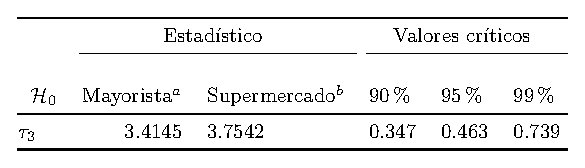
\includegraphics{kpss_12.pdf} 
\caption{con drift}
\end{subfigure}
\begin{subfigure}{\textwidth}
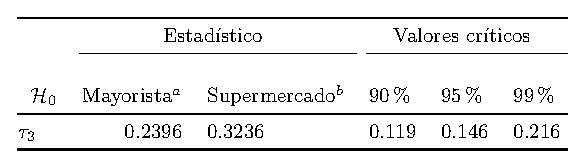
\includegraphics{kpss_11.pdf}
\caption{con drift y tendencia determinista}
\end{subfigure}
\caption*{con cinco rezagos de acuerdo a la regla $\mathbf{lags = \root 4 \of {4 \times (n/100)}}$}
\end{figure}
\end{varwidth}
\end{document}